\documentclass[11pt]{beamer}
\usepackage{listings} % Include the listings-package
\usepackage[T1]{fontenc}
\usepackage[utf8]{inputenc}
\usepackage[english]{babel}
\usepackage{amsmath}
\usepackage{amssymb, amsfonts, latexsym, cancel}
\usepackage{float}
\usepackage{graphicx}
\usepackage{epstopdf}
%\usepackage{subfigure}
\usepackage{hyperref}
%\usepackage{authblk}
\usepackage{blindtext}
\usepackage{booktabs} % Allows the use of \toprule, 
\usepackage{filecontents}
\usepackage{courier} %% Sets font for listing as Courier.
\usepackage{listings}
\usepackage{graphicx}
\usepackage{caption}
\usepackage{subcaption}
\usepackage{graphicx}
\usepackage{subfig}
%\usepackage{listings, xcolor}
\lstset{
tabsize = 2, %% set tab space width
showstringspaces = false, %% prevent space marking in strings, string is defined as the text that is generally printed directly to the console
numbers = left, %% display line numbers on the left
commentstyle = \color{green}, %% set comment color
keywordstyle = \color{blue}, %% set keyword color
stringstyle = \color{red}, %% set string color
rulecolor = \color{black}, %% set frame color to avoid being affected by text color
basicstyle = \small \ttfamily , %% set listing font and size
breaklines = true, %% enable line breaking
numberstyle = \tiny,
}
\usepackage{caption}
\DeclareCaptionFont{white}{\color{white}}
\DeclareCaptionFormat{listing}{\colorbox{gray}{\parbox{\textwidth}{#1#2#3}}}
\captionsetup[lstlisting]{format=listing,labelfont=white,textfont=white}
\definecolor{urlColor}{rgb}{0.06, 0.3, 0.57}
\definecolor{linkColor}{rgb}{0.57, 0.0, 0.04}
\definecolor{fileColor}{rgb}{0.0, 0.26, 0.26}
\hypersetup{
    colorlinks=true,
    linkcolor=linkColor,
    filecolor=fileColor,      
    urlcolor=urlColor,
}
\urlstyle{same}
\setbeamercovered{transparent}
%\usetheme{Boadilla}
\usetheme{CambridgeUS}
%\usetheme{Berkeley}
%\usetheme{Warsaw}
%\usetheme{Madrid}

\title[Experiencia de usuario en portales web]{\bf\Huge Experiencia de usuario en portales web - HCI 2020  }


\author[]
{
    Alvan Ventura Edsel\inst{1}\\
	Chuctaya Ruiz Diego \inst{2}\\
	Esteba Cruz Santos \inst{3}\\
	Ramos Ticona Gilbert\inst{4}
}
\institute[UNSA]
{
\inst{1}% 
System Engineering School\\
}
\date[2020-10-06]{\scriptsize{2020-10-06}}
%\logo{
\includegraphics[width=3.0cm]{img/logo_unsa.jpg}}
\titlegraphic{
\includegraphics[width=1.0cm]{logo_unsa.jpg}}
\begin{document}
    \begin{frame}
    \titlepage
    \end{frame}
    
    
    \begin{frame}
    \frametitle{Content}
    \tableofcontents
    \end{frame}
    
    \section{Accesibilidad}
    \begin{frame}
    \frametitle{Accesibilidad}
    \begin{itemize}
     \item FORMA SIGUE A LA FUNCIÓN.
     \item Objetivo de un portal web es DAR INFORMACIÓN.
    \begin{figure}[t]
    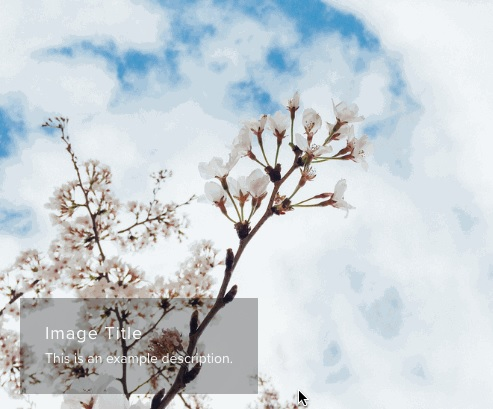
\includegraphics[width=8cm, height=4cm]{over.jpg}
    \centering
    \end{figure}
    \end{itemize}
    \end{frame}
    
    \begin{frame}
    \frametitle{Accesibilidad}
    \begin{itemize}
     \item Popups Escudos de Información.
     \item ¿Con qué finalidad le damos prioridad al diseño que al contenido?
     \end{itemize}
     
     \begin{figure}[t]
    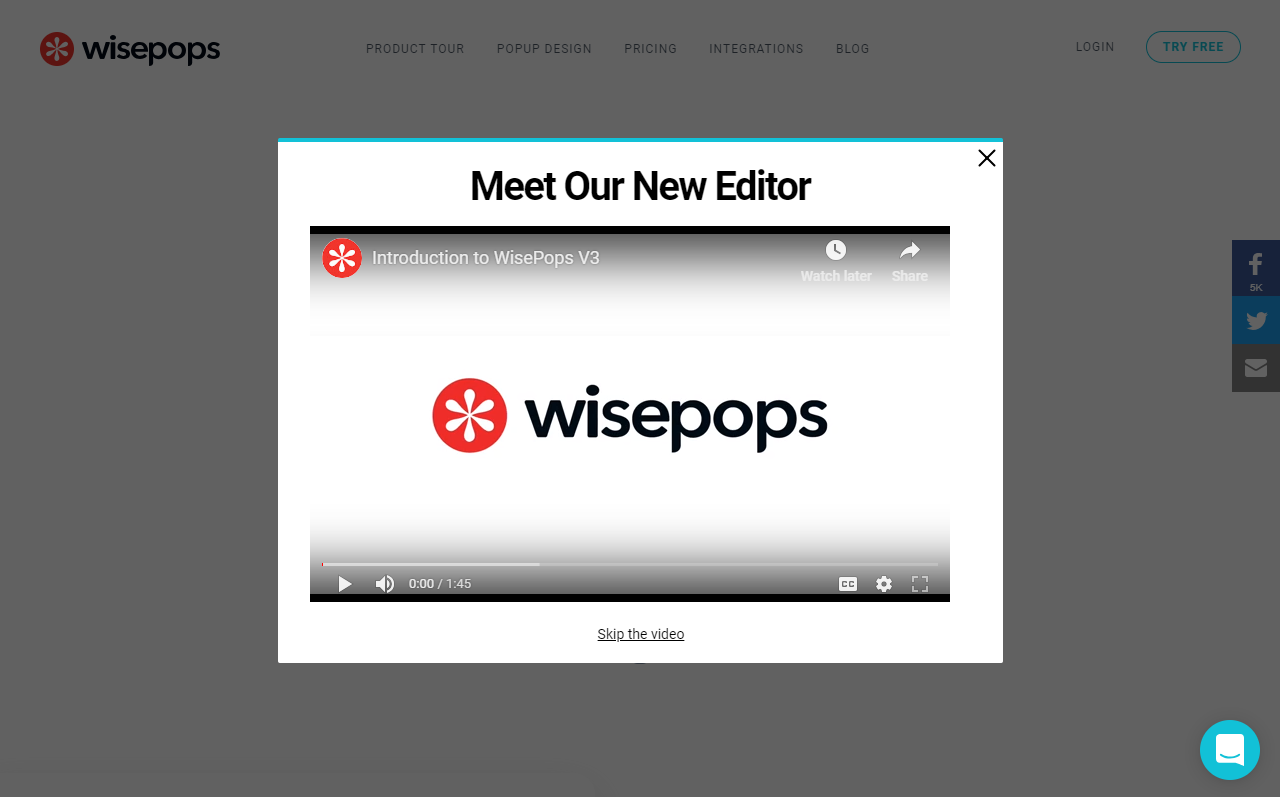
\includegraphics[width=8cm, height=4cm]{pop.png}
    \centering
    \end{figure}
    \end{frame}
    
    
    \section{Navegación}
    %References frame
    \begin{frame}
    \frametitle{Navegación}
    \begin{itemize}
    \item \emph{Se trata de llegar a la información, con la menor cantidad de acciones.}
    \item Amplitud: ¿Cuanta información te muestra, para llegar a la información requerida?
    \item Profundidad: ¿Cuántas acciones haces para llegar a la información?
    \item Breadcrumb("Migas de pan"): ¿Dónde estoy, cómo he llegado hasta aquí y cómo puedo volver atrás o ir a otras páginas similares? 
    
    \begin{figure}[t]
    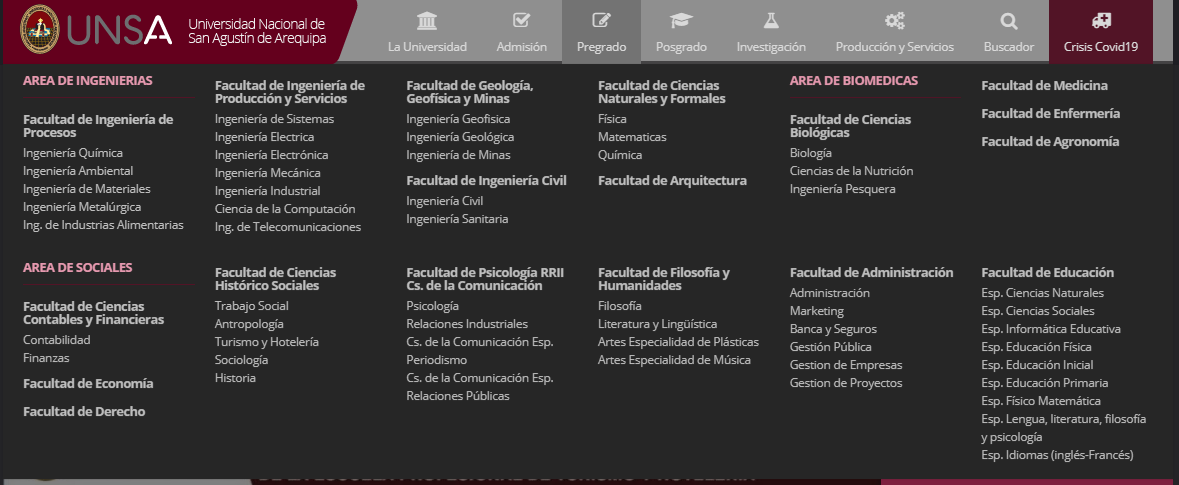
\includegraphics[width=8cm, height=4cm]{unsa_breadcrumbs.PNG}
    \centering
    \end{figure}
    \end{itemize}
    \end{frame}
    
    
    %Menu hamburguesa
    \begin{frame}{Navegación}
        \begin{itemize}
            \item El Menú Hamburguesa: ¿Es bueno o malo?
            \item El menú hamburguesa hace mas dificil el descubrimiento de la información.
            \item Oculta la navegación.
            \item Hay otras formas...
            
           \begin{figure}[!tbp]
                \centering
                \subfloat[macanudo.com]{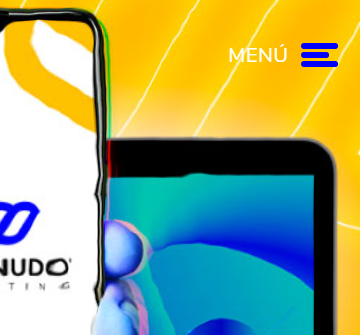
\includegraphics[width=0.3\textwidth,height=4cm]{hamburguesa.PNG}\label{fig:f1}}
                \hfill
                \subfloat[facebook.com]{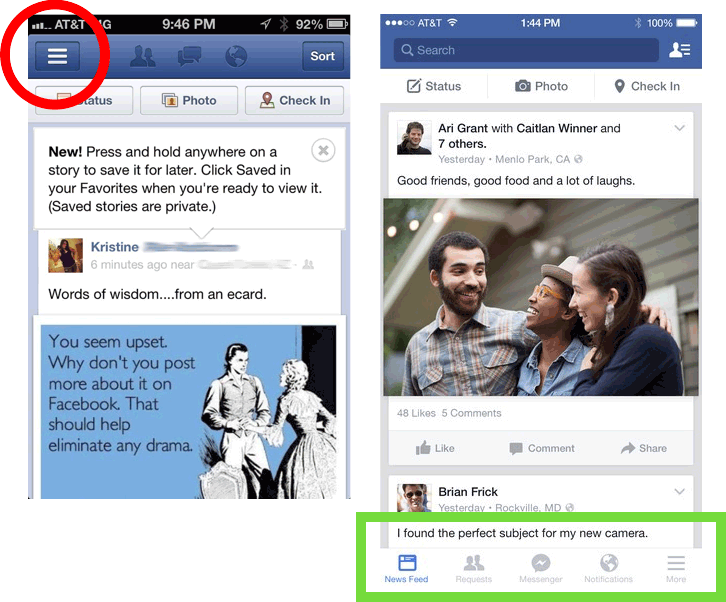
\includegraphics[width=0.6\textwidth,height=5cm]{hamburguesa_2.png}\label{fig:f2}}
            \caption{}
        \end{figure}
        \end{itemize}
    \end{frame}
    
    
    %References contenidos1
    \section{Contenidos}
    \begin{frame}
    \frametitle{Contenidos}
    \begin{itemize}
    \item No importa la cantidad de contenido que le pongas a tu página siempre que la navegación esté bien trabajada.
    \item Los espacios en blanco son parte del diseño.
    \item El contenido antecede al diseño.
    \begin{figure}
        \centering
        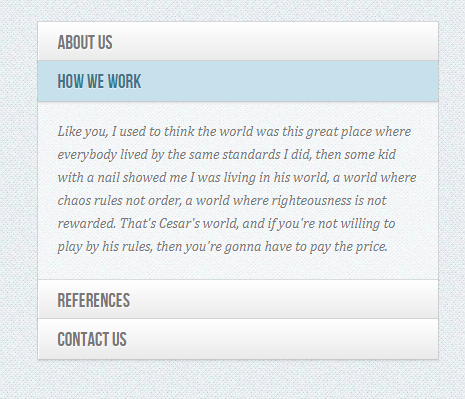
\includegraphics[width=4cm, heigth=5cm]{acordeon.png}
        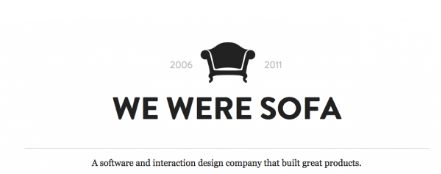
\includegraphics[width=7cm, height=3cm]{blanco.png}
    \end{figure}
    \end{itemize}
    \end{frame}
    
    
    \section{Textos}
    \begin{frame}
    \frametitle{Textos}
    \begin{itemize}
        \item Jerarquías: Normalmente llegan hasta la tercera cabecera y tienen que ser visuales al usuario. 
        \begin{figure}
            \centering
            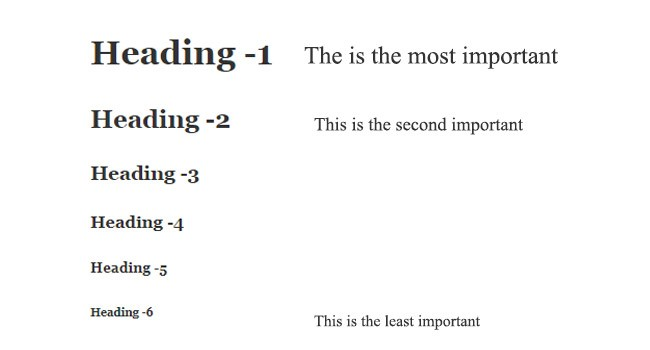
\includegraphics[width=8cm, height=4.5cm]{heading-tags.jpg}
            \caption{Caption}
            \label{fig:my_label}
        \end{figure}
    \end{itemize}
        
    \end{frame}
    
    
    \begin{frame}
    \frametitle{Textos} 
    \begin{itemize}
    \item Alineación: El espacio en un texto justificado no es el mismo , lo que causa que se canse la vista.
    \begin{figure}
        \centering
        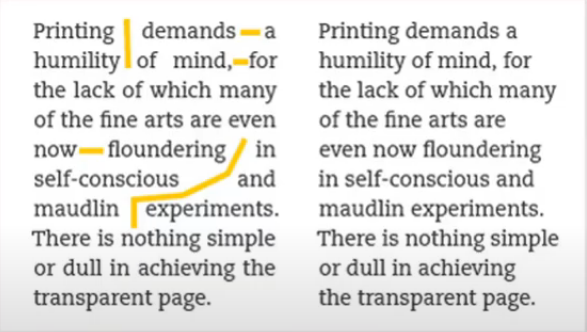
\includegraphics[width=8cm, height=4cm]{con-sin-alineacion.png}
        \caption{Justificación y alineación}
        \label{fig:my_label}
    \end{figure}
    
    \end{itemize}
    \end{frame}
    
    \begin{frame}
    \frametitle{Textos} 
    \begin{itemize}
    \item Alineación
    \begin{figure}
        \centering
        
\includegraphics[width=3cm, height=1.5cm]{sin-alineacion.png}
        \caption{Caption}
        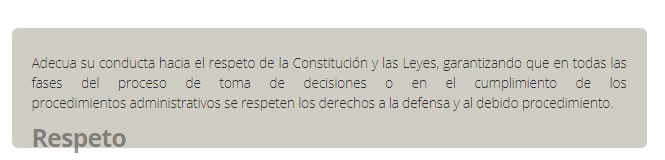
\includegraphics[width=3cm, height=1.5cm]{con-alineacion.png}
        \caption{Caption}
        \label{fig:my_label}
    \end{figure}
    
    \end{itemize}
    \end{frame}
    
    \begin{frame}
    \frametitle{Textos} 
    \begin{itemize}
        \item Ancho de línea ideal: Entre 60 y 70 caracteres de ancho
        \begin{figure}
        \centering
        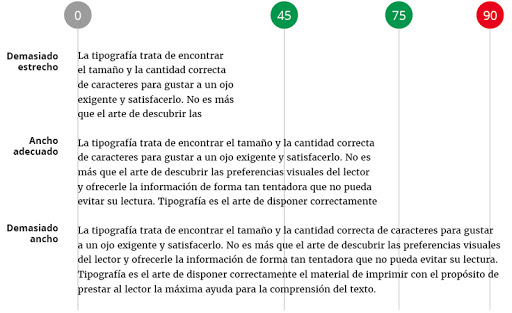
\includegraphics[width=9cm, height=5cm]{ancho-linea.jpg}
        \caption{Ancho de línea ideal}
        \label{fig:my_label}
    \end{figure}
    \end{itemize}
    \end{frame}
    
    \begin{frame}
    \frametitle{Textos} 
    \begin{itemize}
        \item Mayúsculas y minúsculas: Generalmente las mayúsculas se usan para destacar lo más importante.
        \begin{figure}
        \centering
        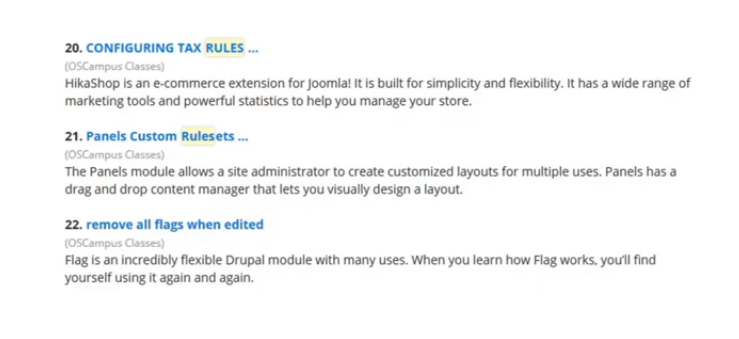
\includegraphics[width=9.5cm, height=5.5cm]{mayus-minus.png}
        \label{fig:my_label}
    \end{figure}
    \end{itemize}
    \end{frame}
    
    
    
    
    
    \section{References}
    %References frame
    \begin{frame}
    \frametitle{References}
    \begin{itemize}
    \item Introduction - XIII, Jhonson J. (2014). Designing with the Mind in mind. 2nd. edition.
    \item Sidney L. Smith and Jane N. Mosier \\
    Albert, A. E. (1982). The effect of graphic input devices on performance in a cursor positioning task. 
    
    \item In Proceedings of the Human Factors Society 26th Annual Meeting (pp. 54-58). Santa Monica, CA: Human Factors Society..
    \end{itemize}
    \end{frame}

\end{document}
